\section{Integrated comparison of endpoint densities}
\label{sec:comparison}

Proposition~\ref{prop:endpoint-matching} compares coefficients and gas
activities. To compare partition functions in volumes growing almost
as fast as $L^{2K}$, we need an estimate with the same small parameter
$\delta_K$. A pointwise relative estimate is unsuitable on configurations
where the signed covering sum is very small. We instead integrate the
comparison before estimating it. The energy released by smoothing a
rough region then pays for its replacement and for the combinatorics
of the covering sum.

Throughout this section $H$ is fixed and large, and
\[
 t=t_0=H^{-1/2}p,\qquad p=p_0=(\log H)^{P_0},\qquad Ht^2=p^2.
\]
We work on standard axis tori of bounded aspect ratio, whose shortest
period exceeds a constant depending on $H$. The periods will also be
required to be multiples of a fixed dyadic integer depending on $H$.
All constants below are independent of the cutoff depth and the periods.

\subsection{The comparison to be proved}

Let $e^X\Xi$ be one of the positive endpoint densities from
Section~\ref{sec:shooting}, with its bulk scalar removed, and write
\[
 Z=\int e^{X(q)}\Xi(q)\,\dd q,
 \qquad \dd\mu(q)=Z^{-1}e^{X(q)}\Xi(q)\,\dd q.
\]
Here $\dd q$ is product normalized area measure on $S^2$. Recall that
$\Xi$ is a mandatory covering sum. For
\[
 D(q)=\{e:|q_x-q_y|>t\},\qquad e=\langle x,y\rangle,
\]
each label $\lambda$ has a fixed nonempty inventory
$J_\lambda$ of bonds, a complete site support $P_\lambda$, and a load
$s_\lambda\ge1$. Its weight vanishes unless
$J_\lambda\subset D(q)$, and its support contains every argument and
every positive or negative eligibility test. A compatible family has
pairwise disjoint supports. Thus
\begin{equation}
 \Xi(q)=\sum_{\substack{\Gamma\ \mathrm{compatible}\\
             \bigsqcup_{\lambda\in\Gamma}J_\lambda=D(q)}}
              \prod_{\lambda\in\Gamma}k_\lambda(q).
 \label{eq:comparison-mandatory-cover}
\end{equation}
In particular $\Xi=1$ if $D(q)$ is empty. This inventory constraint
will be retained in every identity below.

Consider another covering sum $\widetilde\Xi$ on the same inventory
rules, with signed or complex weights allowed. Put unused weights
equal to zero in a common label list, and define
\[
 d_\lambda=\norm{\widetilde k_\lambda-k_\lambda}_\infty,
 \qquad
 p_\lambda=\norm{k_\lambda}_\infty+
                         \norm{\widetilde k_\lambda}_\infty.
\]
The symbol $p_\lambda$ is an activity envelope; the unsubscripted $p$
continues to denote $(\log H)^{P_0}$.

\begin{proposition}[Integrated covering comparison]
\label{prop:integrated-comparison}
Fix any constant multiplier of the covering cap in
Section~\ref{sec:setup}. For sufficiently large $H$, let $e^X\Xi$ be
a standard endpoint density on an axis torus as above, and suppose
\[
 \sup_x\sum_{\lambda:x\in P_\lambda}
                     e^{As_\lambda}p_\lambda
\]
is at most that multiplier times the covering cap. The exponent $A$
is the fixed support exponent of the endpoint class. Then
\begin{equation}
 \frac1Z\int e^X|\widetilde\Xi-\Xi|\,\dd q
 \le \exp\left(\sum_\lambda d_\lambda e^{2s_\lambda}\right)-1.
 \label{eq:orig-16}
\end{equation}
The statement is uniform in cutoff depth and in the admitted periods.
Only the base density $e^X\Xi$ is required to be positive and reflection
positive.
\end{proposition}

The proof has three parts. First, reflection positivity controls the
exponential moment of kinetic energy in any specified set of rows.
Second, rough configurations admit local replacements with a definite
integrated energy gain. Third, exact covering identities organize the
difference into forests to which that gain can be applied.

\subsection{Kinetic energy and a chessboard estimate}

Choose $D_1$ to be an integer comparable with $(\log H)^2$, with a
sufficiently large fixed multiplier. In the kinetic part of $X$,
truncate the exponentially localized kernel $\ell$ at radius $D_1$
using a symmetric truncation. Group the resulting positive square
and the direct term $HS_t$ at each unoriented bond; denote their sum,
including the precise coupling, by $Y_e$. Enlarge the fixed multiple
of $D_1$ when necessary so that it includes every mask read of these
rows. Each $Y_e$ is nonnegative and reads only this finite stencil.

\begin{lemma}[Energy remainder and normalization]
\label{lem:comparison-remainder}
On a terminal torus of volume $v$,
\begin{equation}
 X=-\sum_eY_e+X_{\mathrm{rem}},\qquad
 |X_{\mathrm{rem}}|\le C_Lv,
 \qquad
 |X_{\mathrm{rem}}(q)-X_{\mathrm{rem}}(q')|\le C_Ln
 \label{eq:orig-17}
\end{equation}
whenever $q,q'$ differ at at most $n$ sites. Moreover,
\begin{equation}
 Z\ge e^{-C_Lv\log H},\qquad |\Xi(q)|\le e^v.
 \label{eq:orig-18}
\end{equation}
\end{lemma}

\begin{proof}
Exponential row and column moments bound the omitted kinetic tails.
A change at $n$ sites affects at most $C_LD_1^2n$ mask centers, and
the factor $e^{-cD_1}$ pays for these fixed powers and the coupling.
For the remaining terms, the endpoint bounds in the verification of
\Rref{cmp:RG-density} give canonical size
$C_L(Ht^4+t^2)$ per anchor. Converting the anchor sum to a support-hit
sum costs only a fixed power of $\mathfrak m_0$: complete records
include all graph distances, compensation tags and masks, with the
required load and path moments. The regular errors obey the
corresponding support-hit estimate. Since
$Ht^4+t^2=H^{-1}(p^4+p^2)$, these quantities, even with their fixed
polylogarithmic factors, tend to zero as $H$ increases. This proves
both remainder bounds.

If all spins lie in one cap of radius $cH^{-1/2}$, there are no bad
bonds and $\Xi=1$. The exponent on this cap is bounded below by a
constant times $-v$, while normalized $S^2$ area gives cap measure
at least $c'H^{-1}$ per site. This proves the lower bound for $Z$.
For the other bound, discard compatibility and inventory constraints
only after taking absolute values:
\[
 |\Xi|\le\prod_\lambda(1+\norm{k_\lambda}_\infty)
 \le\exp\left(\sum_\lambda\norm{k_\lambda}_\infty\right)
 \le e^v.
\]
The sums converge by the support-hit cap.
\end{proof}

The chessboard estimate uses the retained seam reflection positivity
from Section~\ref{sec:shooting}; see also the general reflection
positivity framework of \cite{FILS78,FILS80}. We include the finite-tile
argument because later rectangular periods require arbitrary even
tile counts, not only powers of two.

\begin{lemma}[Exponential moments of selected rows]
\label{lem:row-exponential-moment}
Let $B_T$ be a sufficiently large dyadic integer comparable with a
fixed power of $\log H$. On tori whose periods are multiples of
$2B_T$, every set $I$ of unoriented rows satisfies
\begin{equation}
 \E_\mu\exp\left(\theta\sum_{e\in I}Y_e\right)
 \le\exp(C_L|I|B_T^2\log H),
 \qquad \theta=1-C_LD_1/B_T.
 \label{eq:orig-19}
\end{equation}
In particular $B_T$ may be chosen so that $\theta>0$ and
$1-\theta$ is smaller than any prescribed fixed inverse power of
$\log H$.
\end{lemma}

\begin{proof}
For a tiling into $B_T$-squares, let $f_z$ be bounded nonnegative
functions of the sites in tile $z$, with reflected-coordinate
placement denoted by $\theta_zf_z$. The chessboard inequality is
\begin{equation}
 \E_\mu\prod_z\theta_zf_z
 \le\prod_z
 \left(\E_\mu\prod_y\theta_y f_z\right)^{1/N_T},
 \label{eq:comparison-chessboard}
\end{equation}
where $N_T$ is the number of tiles. To prove it for arbitrary even
tile counts, first make the finite collection of tests strictly
positive and normalize each test by its fully disseminated
expectation to the power $1/N_T$. Among all arrays formed from these
normalized tests, choose one maximizing the expectation. Reflection
positivity and Cauchy--Schwarz across any tile seam bound this maximum
by the geometric mean of the expectations of the two reflected
half-arrays. Both half-arrays must therefore also be maximizers.

In one coordinate regard each transverse slab pattern as a letter.
If a longest consecutive run of a letter has length at most half
the cycle, reflect a half containing that run with a seam at one end;
the run grows. If its length exceeds half the cycle, reflect a half
lying within the run and obtain a constant cycle. Repetition makes
the array constant in that coordinate. Repeat in the other
coordinate, preserving the constancy already obtained. Even tile
counts ensure that reflection interchanges the placement conventions
at every seam. A homogeneous normalized array has expectation one,
so the maximum was one. Limits removing the added constants prove
Equation~\eqref{eq:comparison-chessboard} for bounded nonnegative tests.

For a fixed tile grid, retain those rows of $I$ whose complete stencils
lie in a single tile at distance at least $C_LD_1$ from its boundary.
In each occupied tile use the exponential of the sum of its retained
rows as the test. Dissemination gives a subset of the positive rows,
without repetitions, because the stencils remain inside disjoint tiles
and the rows transform covariantly under reflection. If $J$ is such
a disseminated set, Lemma~\ref{lem:comparison-remainder} gives
\[
 \E_\mu e^{\sum_{e\in J}Y_e}
 =Z^{-1}\int
 e^{-\sum_{e\notin J}Y_e+X_{\mathrm{rem}}}\Xi\,\dd q
 \le e^{C_Lv\log H}.
\]
The chessboard norm of an occupied tile consequently costs at most
$e^{C_LB_T^2\log H}$. There are at most $|I|$ occupied tiles.

Finally average over all $B_T^2$ translations of the tile grid.
Every row is retained for at least a fraction
$1-C_LD_1/B_T$ of these translations. Since $Y_e\ge0$, generalized
Hölder applied to the corresponding grid estimates yields
Equation~\eqref{eq:orig-19}.
\end{proof}

\subsection{Regions that can be replaced at an energy gain}

Use max distance on the torus, put
\[
 f(x)=\max_{e\ni x}|q_x-q_y|,
 \qquad a=\varepsilon t,
\]
and choose $\varepsilon>0$ sufficiently small, independently of $H$.
Mark every site of every integer square box of radius at most one
fourth of the shortest period, including radius zero, on which the
average of $f$ exceeds $a$. Let $U$ be the union of all marked boxes.
Dilate $U$ by $d=CD_1$, take its max-neighbor connected components,
and retain the complete components containing a true bad bond
$|q_x-q_y|>t$. Denote them by $E_C$. Distinct retained components have
nonadjacent sites, and every true bad bond lies deep inside exactly
one retained component. The construction is illustrated in
Figure~\ref{fig:editable}.

\begin{figure}[htbp]
\centering
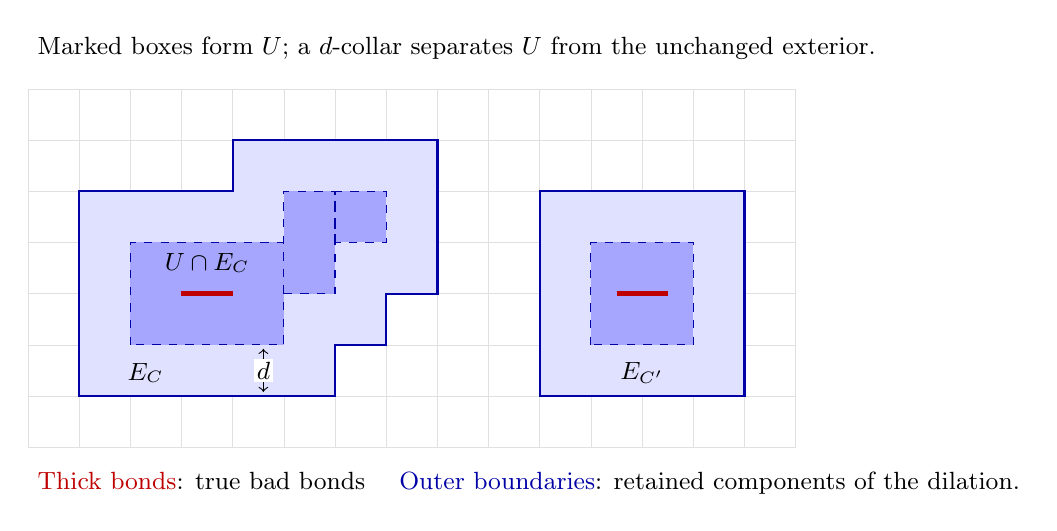
\begin{tikzpicture}[x=0.65cm,y=0.65cm,font=\small]
  \draw[step=1,black!12,very thin] (0,0) grid (15,7);
  \fill[blue!12] (1,1) -- (6,1) -- (6,2) -- (7,2) -- (7,3) -- (8,3) -- (8,6)
      -- (4,6) -- (4,5) -- (1,5) -- cycle;
  \draw[blue!65!black,thick] (1,1) -- (6,1) -- (6,2) -- (7,2) -- (7,3) -- (8,3)
      -- (8,6) -- (4,6) -- (4,5) -- (1,5) -- cycle;
  \fill[blue!35] (2,2) rectangle (5,4);
  \fill[blue!35] (5,3) rectangle (6,5);
  \fill[blue!35] (6,4) rectangle (7,5);
  \draw[blue!65!black,dashed] (2,2) rectangle (5,4);
  \draw[blue!65!black,dashed] (5,3) rectangle (6,5);
  \draw[blue!65!black,dashed] (6,4) rectangle (7,5);
  \fill[blue!12] (10,1) rectangle (14,5);
  \draw[blue!65!black,thick] (10,1) rectangle (14,5);
  \fill[blue!35] (11,2) rectangle (13,4);
  \draw[blue!65!black,dashed] (11,2) rectangle (13,4);
  \draw[red!75!black,line width=2pt] (3,3) -- (4,3);
  \draw[red!75!black,line width=2pt] (11.5,3) -- (12.5,3);
  \node at (2.3,1.45) {$E_C$};
  \node at (12,1.45) {$E_{C'}$};
  \node at (3.5,3.6) {$U\cap E_C$};
  \draw[<->] (4.6,1.08) -- (4.6,1.92);
  \node[fill=white,inner sep=1pt] at (4.6,1.5) {$d$};
  \node[anchor=west,align=left] at (0,7.8)
      {Marked boxes form $U$; a $d$-collar separates $U$ from the unchanged exterior.};
  \node[anchor=west] at (0,-0.7)
      {\textcolor{red!75!black}{Thick bonds}: true bad bonds \quad
       \textcolor{blue!65!black}{Outer boundaries}: retained components of the dilation.};
\end{tikzpicture}
\caption{Schematic editable regions. Each dark region is a union of
marked boxes, and each light region is the complete connected component
of its $d$-dilation. The replacement uses all sites of a selected light
region. Its outer collar lies outside $U$, so it joins the unchanged
configuration without creating a bad bond. Distinct retained components
have nonadjacent sites. The drawing suppresses lattice boundary
conventions and is not to scale.}
\label{fig:editable}
\end{figure}

\FloatBarrier

\begin{lemma}[Replacement and its energy bounds]
\label{lem:editable-regions}
The constants $\varepsilon$ and $C$ can be chosen so that the
following statements hold for all sufficiently large $H$ and
sufficiently large admitted periods.
\begin{enumerate}[label=\textup{(\roman*)}]
\item The unchanged values on $U^c$ have a measurable extension to all
sites in $S^2$ with nearest-neighbor chords at most $C'a$. For each
region $E_C$, independently sampling every spin in a cap of radius
$c't$ about this extension removes all its true bad bonds and creates
none. Any subset of the regions may be replaced in this way. The
conditional sampling density for $n$ replaced sites is at most
$\exp(Cn\log H)$ with respect to product normalized area measure.
\item For a union $E$ of selected regions, let $n=|E|$. There is a set
$I_E$ of rows, consisting of all rows within distance $C'D_1$ of $E$,
which includes every changed kinetic stencil and satisfies
$|I_E|\le Cd^2n$. Its total stencil enlargement is less than $d/2$.
For the original configuration and every sampled replacement $q'$,
\begin{align}
 \sum_{e\in I_E}Y_e(q)&\ge cp^2n/d^2,
 \label{eq:orig-20}\\
 \sum_{e\in I_E}Y_e(q')&\le C_Ld^2p^2n.
 \label{eq:orig-21}
\end{align}
\end{enumerate}
\end{lemma}

\begin{proof}
We first establish the exterior Lipschitz estimate. At a point of
$U^c$, every allowed box containing that point has average gradient
at most $a$. Compare the spin at the point with averages over
successive concentric doubled boxes. The discrete $L^1$ Poincar\'e
inequality, obtained by summing coordinate paths, bounds the change
at scale $R$ by $CR$ times the average gradient on a fixed enlargement.
For two points, stop at the scale of their separation and compare the
two averages through an enclosing box of comparable size. Summing
the geometric scales gives
\[
 |q_x-q_y|\le Ca\,\operatorname{dist}(x,y),\qquad x,y\in U^c.
\]
The radius-one case uses the same coordinate-path estimate. If the
required scale exceeds the allowed box size, the sphere's bounded
diameter proves the estimate once the shortest period is much larger
than $a^{-1}$.

Extend these exterior data componentwise to an $O(a)$-Lipschitz
Euclidean-vector-valued function on the continuous torus, using
distance cones. Within distance $c/a$ of the prescribed data the
extension has norm bounded away from zero; normalization therefore
gives an $S^2$-valued extension there with Lipschitz constant $O(a)$.
Choose a torus mesh of width comparable with $c'/a$, where $c'$ is
sufficiently smaller than $c$. Preserve this extension in every mesh
box meeting the prescribed data. Choose a common arbitrary spin at
all remaining undetermined vertices, and use measurably selected
shortest arcs on the undetermined mesh edges.

Each remaining box now has a boundary map into $S^2$ with uniformly
bounded Lipschitz constant after rescaling. To fill it, cover the
antipodal image curve by $O(1/\tau)$ spherical balls of radius $\tau$.
Their total area is $O(\tau)$, so for a sufficiently small fixed $\tau$
there is a point $p_*$ uniformly separated from the antipodal curve.
If the boundary map in disk coordinates is $g(\theta)$, the normalized
cone
\[
 F(r,\theta)=
 \frac{(1-r)p_*+rg(\theta)}{|(1-r)p_*+rg(\theta)|}
\]
has a uniform Lipschitz bound. A fixed bi-Lipschitz change between a
disk and a square preserves that bound. This is the filling argument
of \Rref{cmp:filling}, with the area of $S^2$ replacing the volume of
$S^3$. Adjacent fillings agree on their already chosen edges. Fixed
ordered nets for $p_*$ and measurable arc choices make the construction
measurable. The same construction works if there are no exterior data.
Rescaling gives the claimed $C'a$ bound.

Choose $\varepsilon$ so that this bound is a sufficiently small
fraction of $t$. Choose the sampling cap radius $c't$ smaller still.
All sampled adjacent spins then have chords below $t$. A boundary
edge of a retained region lies in the collar outside $U$, where the
extension equals the unchanged data; thus crossing edges also remain
below $t$. Every originally true bad bond belongs to a retained
region. Consequently replacing any selected regions removes exactly
their bad-bond inventories. A cap of radius $c't$ on $S^2$ has area
at least $ct^2$, so its normalized sampling density is at most
$C/t^2\le H^C$. Taking products proves the density bound.

For the lower energy estimate, select disjoint generating marked
boxes in each component, in decreasing order of size. Fixed
enlargements of the selected boxes cover all generating boxes.
Dilation by $d$ enlarges the area of a unit or larger box by at most
$Cd^2$. The total selected area in $E_C$ is therefore at least
$c|E_C|/d^2$. On each selected box the average of $f$ exceeds $a$.
If this average is supplied mainly by chords greater than $t$, the
positive linear branch of $S_t$ gives an energy lower bound
$cHa^2$ times the box area. Otherwise Cauchy--Schwarz in the quadratic
branch gives the same lower bound. Bonds incident to disjoint selected
boxes are counted at most a bounded number of times. Since
$Ha^2=\varepsilon^2p^2$, summation proves
Equation~\eqref{eq:orig-20}.

Choose the fixed multiple in $d=CD_1$ after the stencil constants, so
that all stencils read by rows of $I_E$ stay within a $d/2$ enlargement
of $E$. On the replaced sites all chords are below $t$. Any
unselected component of the full dilated construction has its
original marked part at distance at least $d$ from $E$; elsewhere
the unchanged chords are bounded by the exterior estimate. Thus
every chord read by these rows is at most $t$. Uniform summability of
the row weights gives $Y_e(q')\le C_LHt^2=C_Lp^2$.
The support count $|I_E|\le Cd^2n$ proves
Equation~\eqref{eq:orig-21}.
\end{proof}

The lower bound is proportional to the number of replaced sites,
with only the polylogarithmic loss $d^2$. This is what allows an
integrated estimate uniform in the total volume. Fix $B_T$ in
Lemma~\ref{lem:row-exponential-moment} so large that
\begin{equation}
 (1-\theta)C_Ld^2<\frac{c}{4d^2},
 \label{eq:comparison-theta-choice}
\end{equation}
with the constants of Lemma~\ref{lem:editable-regions}. Next take
$P_0$ sufficiently large that
\begin{equation}
 p^2/d^2\gg d^2B_T^2\log H+\log H+1.
 \label{eq:comparison-p-choice}
\end{equation}
All powers on the right were fixed independently of $P_0$. These
requirements can therefore be included among the finite choices
before taking $H$ large.

\subsection{Exact covering identities and integration}

We now keep the geometry of the original configuration fixed while
removing selected inventories. This distinction is important: no
modified configuration is reclustered.

Let $\mathcal I$ be the family of retained regions of a configuration
$q$, and let $D_C$ be the original true bad bonds assigned to $E_C$.
Choose filled values at every region as in
Lemma~\ref{lem:editable-regions}. For $I\subset\mathcal I$, let $q(I)$
be the configuration in which precisely the regions outside $I$ have
been replaced. Then
\begin{equation}
 D(q(I))=\bigsqcup_{C\in I}D_C.
 \label{eq:comparison-inventory-edit}
\end{equation}
Write $\Xi(I)=\Xi(q(I))$; these are complete positive sums.

At a fixed active set $I$, join two labels of a full covering family
if their supports meet the same active region. Call a connected group
a macrolabel $U$. Its enlarged support and weight are
\[
 S_U=\bigcup_{\lambda\in U}P_\lambda
 \ \cup\!
 \bigcup_{\substack{C\in I:\ E_C\cap P_\lambda\ne\varnothing\\
                                  \text{for some }\lambda\in U}}E_C,
 \qquad
 w(U;q(I))=\prod_{\lambda\in U}k_\lambda(q(I)).
\]
All labels supplying the inventory of a touched region belong to the
same group, so each macrolabel covers every active region it meets
in full. Distinct macrolabels have disjoint enlarged supports.
Conversely, compatible macrolabels covering the active inventories
recover a full original covering family.

If a site set $S$ is disjoint from the active regions, denote by
$\Xi(I;S)$ the complete-inventory sum restricted to macrolabels
whose enlarged supports avoid $S$. This restricted sum may be signed.
For a selected compatible macrolabel family $\mathcal A$, let
$S_{\mathcal A}$ be its combined support and $B_{\mathcal A}$ the
active regions it covers. The exact identities from
\Rref{cmp:background-identity}, \Rref{cmp:IE}, and
\Rref{cmp:difference-identity} become
\begin{align}
 \Xi(I;S)
 &=\sum_{\substack{\mathcal A\ \mathrm{compatible}\\
          S_U\cap S\ne\varnothing\ (U\in\mathcal A)}}
 (-1)^{|\mathcal A|}
 \prod_{U\in\mathcal A}w(U;q(I))\,
 \Xi(I\setminus B_{\mathcal A};S_{\mathcal A}),
 \label{eq:comparison-inclusion-exclusion}\\
 \widetilde\Xi(I)-\Xi(I)
 &=\sum_{\substack{\mathcal A\ \mathrm{compatible}\\
                              \mathcal A\ne\varnothing}}
 \prod_{U\in\mathcal A}
       [\widetilde w(U;q(I))-w(U;q(I))]\,
 \Xi(I\setminus B_{\mathcal A};S_{\mathcal A}).
 \label{eq:comparison-difference-identity}
\end{align}
Here and below macrolabels in a displayed sum satisfy the inventory
conditions just described.

To verify the identities, first select a compatible family. Every
remaining support avoids $S_{\mathcal A}$ and hence every changed
site. Its values and all eligibility indicators are unchanged by
removing $B_{\mathcal A}$. Its inventory loses exactly the removed
inventories in Equation~\eqref{eq:comparison-inventory-edit}. This
gives the background sum
$\Xi(I\setminus B_{\mathcal A};S_{\mathcal A})$.
Expand the indicator of avoiding $S$ as a product of
$1-\mathbf1_{\{S_U\cap S\ne\varnothing\}}$ to obtain the first
identity. Expand $\widetilde w=w+(\widetilde w-w)$ in a full family
and subtract the all-$w$ term to obtain the second. With finite label
lists these are finite algebraic identities. A full family contains
at most $|D(q(I))|$ labels, and the absolute activity bounds give
convergence for countable lists, so the identities pass to that
limit before any division is performed.

Starting with Equation~\eqref{eq:comparison-difference-identity},
iterate Equation~\eqref{eq:comparison-inclusion-exclusion} until
each term ends in a complete base sum $\Xi(q')$. Every nonempty
generation consumes an active region, so this recursion terminates.
Fix an ordering of the common label list. Take absolute values and
telescope each initial macrolabel difference in this order:
\begin{equation}
 |\widetilde w(U)-w(U)|
 \le\sum_{\lambda\in U}d_\lambda
             \prod_{\kappa\in U\setminus\{\lambda\}}p_\kappa.
 \label{eq:comparison-marked-product}
\end{equation}
Thus each initial macrolabel has one marked original label, carrying
$d_\lambda$; the other labels carry $p_\lambda$. The final complete
$\Xi(q')$ is positive.

We record explicitly the gain after integrating such a term. A term
will be encoded below by its original labels and the exact site sets
of its consumed regions. Fix these sets, let their union be $E$, and
put $n=|E|$. Let $\mathcal Q$ be the measurable set of original
configurations whose region construction and original inventories admit
this encoded term. Label lists include zero-valued labels: every
spin-dependent eligibility test remains in the evaluated weight. Thus
$\mathcal Q$ is defined before sampling, even when a later evaluated
weight vanishes for some filled values. Average over the sampled
filled values; only consumed regions need to be sampled. Then
\begin{equation}
 \frac1Z\int_{\mathcal Q} e^{X(q)}
           \E_{\mathrm{fill}\mid q}[\Xi(q')]\,\dd q
 \le e^{-c'p^2n/d^2}.
 \label{eq:orig-22}
\end{equation}
Indeed Equations~\eqref{eq:orig-17} and~\eqref{eq:orig-20} imply
\[
 X(q)-X(q')\le C_Ln-cp^2n/d^2+\sum_{e\in I_E}Y_e(q').
\]
By Equation~\eqref{eq:orig-21} and the choice
\eqref{eq:comparison-theta-choice}, replacing the last coefficient
one by $\theta$ costs at most $cp^2n/(4d^2)$.

There is no change-of-variables invertibility assumption here.
Write $q=(q_E,q_{E^c})$ and let
$h(q'_E\mid q_E,q_{E^c})$ be the conditional fill density. Its
uniform bound is $e^{Cn\log H}$. After using that bound, positivity
of $\Xi(q')$ allows the restrictions defining $\mathcal Q$ to be
dropped. Integration over the original $q_E$ contributes at most
one, since it uses product probability measure. The remaining
integral over $(q'_E,q_{E^c})$ is bounded by
\[
 \exp\left(C_Ln+Cn\log H-\frac{3cp^2n}{4d^2}\right)
 \E_\mu\exp\left(\theta\sum_{e\in I_E}Y_e\right).
\]
Equation~\eqref{eq:orig-19}, $|I_E|\le Cd^2n$, and
Equation~\eqref{eq:comparison-p-choice} prove
Equation~\eqref{eq:orig-22}. This is the only integration estimate
needed in the covering recursion; no restricted signed sum appears
in a denominator.

\subsection{Summing the forests}

We complete the proof of Proposition~\ref{prop:integrated-comparison}
by explaining the counting in \Rref{cmp:forest} for these regions.
Inside each macrolabel choose a spanning tree on its original label
nodes and the active-region nodes it meets. Make the choice
deterministically using a fixed ordering. Join each later macrolabel,
again deterministically, to one preceding-generation macrolabel whose
support it meets. Choose a deterministic intersecting pair of their
underlying gas or region supports as the endpoints of this edge. Use
two edge colors to distinguish edges internal
to a macrolabel from edges joining generations, and root each tree
at the marked label of its initial macrolabel.

No region node is repeated: a region is consumed on first appearance.
No original label is repeated either. Its inventory is fixed and
nonempty, and the regions containing it have already been removed
after its first appearance. It cannot be eligible in a subsequent
generation. Within a generation the supports are disjoint.

This forest retains the entire term. Contracting internal edges
recovers the macrolabels; depths in the contracted rooted forest
recover generations; marked roots recover the telescoping choices.
The exact region site sets recover the consumed active sets and
therefore every evaluation configuration. Thus distinct terms do
not acquire the same forest. For a fixed original configuration the
unconsumed geometry and inventories are already determined; there
is no further multiplicity to count.

After integration, Equation~\eqref{eq:orig-22} assigns an edit node
$E_C$ the weight
\[
 w(E_C)=e^{-c'p^2|E_C|/d^2}.
\]
Since the consumed sets are disjoint, their product is exactly the
weight for their union. We may now enlarge the possible geometries
to all connected site animals. On a bounded-degree lattice the number
of animals of size $n$ containing a fixed site is at most $C^n$;
the same bound follows by a spanning-tree traversal on a torus.
Consequently, with $R=C_L\mathfrak m_0^2$ large enough that
$|P_\lambda|\le Rs_\lambda$,
\[
 \sup_x\sum_{E_C:x\in E_C}w(E_C)e^{2|E_C|}
 \le\sum_{n\ge1}C^ne^{-(c'p^2/d^2-2)n}
 <\frac1{16R}
\]
for sufficiently large $H$. The activity cap likewise gives
\[
 \sup_x\sum_{\lambda:x\in P_\lambda}
                    p_\lambda e^{2s_\lambda}<\frac1{16R}.
\]
Indeed $A=64\ge2$ and $Rw_0\to0$, even after multiplying the cap by
any fixed constant, by Equation~\eqref{eq:setup-covering-norm}.
Give a gas node size $s_\lambda$ and an edit node size $|E_C|$.
Every node of size $b$ has support at most $Rb$. Summing over an
intersection site and the two edge colors bounds the one-child sum,
with an exponential allowance for descendants, by $b/4$.

More explicitly, induction on maximum tree depth bounds the total
descendant weight below a root of size $b$ by $e^b$. For the induction
step, a child of size $a$ contributes at most its weight times $e^a$.
The sum over unordered distinct children is bounded by the
exponential of the one-child sum, because ordered $r$-tuples with
factor $1/r!$ only enlarge it after distinctness is dropped. Hence
the descendant sum is at most $e^{b/4}\le e^b$. Monotonicity of the
positive majorants allows arbitrary depth.

A marked gas root therefore costs at most
$d_\lambda e^{s_\lambda}\le d_\lambda e^{2s_\lambda}$.
Actual forest components have distinct marked roots. Dropping all
disjointness conditions between their descendant trees and summing
unordered nonempty root sets gives
\[
 \sum_{r\ge1}\frac1{r!}
 \left(\sum_\lambda d_\lambda e^{2s_\lambda}\right)^r.
\]
This is the right-hand side of Equation~\eqref{eq:orig-16}, proving
Proposition~\ref{prop:integrated-comparison}.

\subsection{Partition functions and ordinary alignment}

Apply Proposition~\ref{prop:integrated-comparison} to the two endpoint
gases in Equation~\eqref{eq:orig-15}. Summing their support-hit bound
over sites gives
\[
 \sum_\lambda d_\lambda e^{2s_\lambda}\le D_Hv\delta_K.
\]
The exponent comparison in that equation then shows that the ratio
of the scalar-stripped partition functions tends to one whenever
$v\delta_K\to0$. For example, with $\varepsilon_K=D_Hv\delta_K$,
\[
 \left|\frac{\int e^{X_1}\Xi_2}{\int e^{X_1}\Xi_1}-1\right|
 \le e^{\varepsilon_K}-1,
 \qquad
 e^{-\varepsilon_K}\le e^{X_2-X_1}\le e^{\varepsilon_K}.
\]
For small $\varepsilon_K$ these inequalities bound the logarithm of
the partition-function ratio by $C\varepsilon_K$. The constants
depend on the fixed $H$, but not on depth or period. The same
integrated estimate will also be used when activity differences
are localized at specified source sites, in which case their sum
does not carry a factor $v$.

We also need a local consequence of reflection positivity.

\begin{corollary}[Terminal alignment]
\label{cor:terminal-alignment}
On every standard terminal axis torus considered in this section,
for each fixed $C>0$ there is $c>0$ such that every bond satisfies
\begin{equation}
 \mu\{|q_x-q_y|>t/C\}\le e^{-cHt^2}.
 \label{eq:orig-23}
\end{equation}
The constants are uniform in the cutoff depth and the admitted periods.
\end{corollary}

\begin{proof}
Choose a translated $2$-by-$2$ tile containing the specified bond and
disseminate its event by tile reflections. The periods are divisible
by $2B_T$, hence by $4$, so these tiles have even counts in both
directions. A fixed positive fraction of all bonds then have chord
greater than $t/C$.
The direct kinetic energy on that event is at least $cHt^2v$.
Equations~\eqref{eq:orig-17} and~\eqref{eq:orig-18} bound its
probability by
\[
 \exp[-v(cHt^2-C_L-C_L\log H)]\le e^{-c'vHt^2}.
\]
The chessboard inequality gives the single-event bound after taking
the corresponding tile root. This is the argument of
\Rref{cmp:rarity}, whose hypotheses have now all been checked for
the $S^2$ endpoint law. No such estimate is used in oblique periods.
\end{proof}
